\myframe{Cafer Paşa}{frame:cafer}{
  \setfarsi
  \novocalize
  \only<1>{
    \begin{center}
      \begin{tabular}{l@{\hspace{2cm}}r}
        \multicolumn{2}{c}{\includegraphics[scale=0.15]{parole/cafer.png}}\\
        Cafer, Mîr-i  mîrler-i Kıbrıs  & \RL{^g`fr mIri  mIrlar qubris}\\[1cm]
        \multicolumn{2}{c}{\footnotesize Cafer Paşa,  governatore di Cipro (vari mandati  dal 1003/1595).}\\[2mm]
        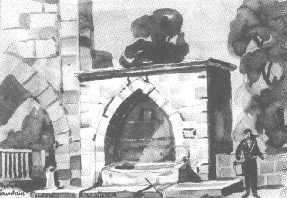
\includegraphics[scale=0.3]{atlas/cafer-fontana.png}
        &  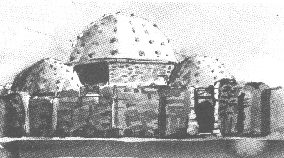
\includegraphics[scale=0.3]{atlas/cafer-bagno.png} \\
        1597 
        & 1601 \\
      \end{tabular}
    \end{center}
  }
  \only<2>{
    \begin{center}
      \begin{tabular}{p{0.48\textwidth}p{0.48\textwidth}}
        {\centering\includegraphics[scale=0.3]{documenti/vecellio295.png}}&
        {\centering\includegraphics[scale=0.4]{ritratti/Nadiri_f_8_v.jpg}}\\ 
        
        {\centering\tiny {\sc Cesare Vecellio}, {\it Habiti antichi et moderni
            di tutto il mondo}, Venezia, 1598}
        
        & {\centering\tiny
            {\it  Musicisti di fronte  a Mehmed  III}, Topkapı  Sarayı Müzesi,
            inv.  H889, f.  8, XVII  sec.} \\
      \end{tabular}
    \end{center}
  }

  \only<3>{
    \begin{center}
      \begin{tabular}{cc}
        \includegraphics[scale=0.25]{foto/aleppo-room-pergamon-1.png} &
        \includegraphics[scale=0.25]{foto/aleppo-room-pergamon-2.png} \\[1cm]
        \multicolumn{2}{c}{\tiny {\it Sala di Aleppo}, 1600-01, 
          Museums für Islamische Kunst (Pergamon), Berlin}\\ 
      \end{tabular}
    \end{center}
  }

}

\myincslide{frame:cafer}{2}
\myincslide{frame:cafer}{3}

\mode
<article>

Cafer Paşa si firma come  \RL{mIri mIrlar qubris}, {\it Mîr-i mîrler-i
  Kıbrıs},  ossia governatore di  Cipro. In  realtà, lui  stesso nella
lettera dice di esserlo stato in passato, lasciando sottindere che non
lo è più in questo momento.

Cafer  Paşa sarà  comunque spesso  governatore di  Cipro negli  anni a
cavallo  del  1600 (dal  1003/1595  al  1038/1629),  anche in  periodi
successivi  a  questa  lettera   \cite[p.  9]{sengor}.  A  Cipro  farà
costruire  tra   le  altre  cose   un  bagno  (1601)  e   una  fontana
(1597). Muore intorno al 1620.

Il  termine consueto  per  governatore sarebbe  \RL{mIri mIrAn},  {\it
  Mîr-i mîran}  \cite[p. 6]{sengor}. Tuttavia qui, come  in altri casi
all'interno della lettera,  Cafer Paşa non usa il  plurale persiano in
\RL{BAn}, {\it -an}, ma quello turco in \RL{Blar}, {\it -lEr}.

Da notare che il dragomanno traduce il titolo con Beylerbey.

\mode
<all>

\myframet{Muhibbane inha}{Inha}{frame:muhibbane}{

  \mbox{ }
  \vfill

  \parbox[c]{0.4\textwidth}{
    \begin{tabular}{c}
      \includegraphics{parole/muhibbane.png}\\
      \RL{mu.hibbAnah  in.hA}\\[1cm]
      muhibbane inha\\[1cm]
    \end{tabular}}
  \hfill
  \parbox[c]{0.55\textwidth}{
    \begin{tabular}{c}
      \includegraphics[scale=0.1]{documenti/frammento.png}\\[2mm]
      {\tiny ASVE, {\it Documenti Turchi}, n. 1099}\\[1cm]
      \includegraphics[scale=0.1]{documenti/doc1050.png}\\[2mm]
      {\tiny ASVE, {\it Documenti Turchi}, n. 1050}\\[1cm]
    \end{tabular}}

  \vfill
}

\myframe{Venedik Duzı}{frame:venedikduzi}{

\setarab
\novocalize
\begin{center}
\begin{tabular}{lr}
  \multicolumn{2}{c}{\includegraphics{parole/venedik_duzi.png}}\\
  Venedik duzı & \RL{wenedIk dUzI}\\[1cm]
  \multirow{2}{*}{\includegraphics[scale=0.28]{ritratti/marino_grimani.jpg}}&
    Marino Grimani\\
    &1532-1605, doge dal 1595\\[2cm]
    &\parbox{0.3\textwidth}{\tiny Gabriele Caliari, {\it Il doge Marino Grimani riceve l'ambasciatore persiano}, Venezia, Palazzo Ducale, XVI sec.}\\
\end{tabular}
\end{center}
\setfarsi
}

\mode
<article>

Cafer Paşa scrive al Doge di Venezia, all'epoca Marino Grimani.\cite{itmarinogrimani}

\mode
<all>

\myframe{Kıbrıs}{frame:kibris}{
\setarab
\novocalize
\begin{center}
\begin{tabular}{l@{\hspace{2cm}}r}
  \multicolumn{2}{c}{\includegraphics{parole/kibris_vilayet.png}}\\
  bu muhibları vilâyet Kıbrıs
  & \RL{bU mu.hiblarY wilAyat qubris}\\[1cm]
  \multicolumn{2}{c}{
    \parbox[c]{0.58\textwidth}{\centering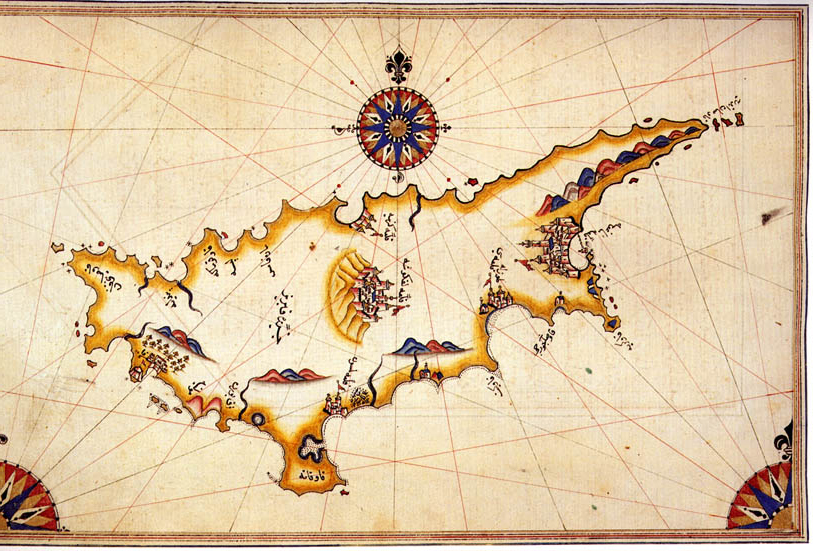
\includegraphics{atlas/Cyprus_by_Piri_Reis.jpg}}
    \parbox[c]{0.35\textwidth}{\tiny {\sc Piri Reis}, {\it Kitab-ı Bahriye}, 1521-25}}\\
\end{tabular}
\end{center}
}

\myframe{Yaqumu Biazii}{frame:yaqumu}{
\setfarsi
\novocalize
\parbox[c]{0.48\textwidth}{
  \begin{tabular}{c}
    \includegraphics{parole/yaqum_biazii.png}\\
    \RL{yaqumU byAzY nAm}\\
    Yaqumu Biazii nam\\[0.5cm]
    \includegraphics{parole/rayetinize.png}\\
    \RL{ra`iyatikizah}\\
    ra`iyetinize\\
\end{tabular}}\hfill\parbox[c]{0.5\textwidth}{\centering
  \begin{tabular}{p{0.48\textwidth}}
    \includegraphics[scale=0.3]{documenti/vecellio321.png}
    \includegraphics[scale=0.3]{ritratti/mercante2.png}\\[0.2cm]
    {\tiny {\sc Cesare Vecellio}, {\it Habiti antichi et moderni di tutto il mondo}, Venezia, 1598}\\
  \end{tabular}}
}

\mode
<article>

Nella lettera racconta che,  quand'era a Cipro come governatore, aveva
conosciuto  un tal  \RL{yaqumU  byAzY}, {\it  Yaqumu Biazii}  (Giacomo
Biasii), nel quale  lui riponeva fiducia. Questo Biasii  è indicato al
doge  come \RL{ra`iyatikizah},  {\it ra`iyetinize},  cioè  {\it vostro
  suddito}. Si tratta quindi di un veneziano.

\mode
<all>

\myframe{Penbe}{frame:penbe}{
  \setfarsi
  \novocalize
  \parbox[c]{0.4\textwidth}{\centering\begin{tabular}{c}
      \includegraphics{parole/penbe.png}\\[1cm]
      \RL{panbah}\\[1cm]
      penbe\\
  \end{tabular}}
  \hfill\parbox[c]{0.55\textwidth}{
    \begin{tabular}{c}
      \includegraphics[scale=0.6]{documenti/alpino.jpg}\\
      {\tiny {\sc Prosper Alpinus}, {\it De Plantis Aegypti Liber}, Venezia 1592}\\
  \end{tabular}}
}

\myframet{Agnello vegetale}{A. vegetale}{frame:agnellovegetale}{
  \setfarsi
  \novocalize
  \tiny
  \begin{tabular}{cp{0.5\textwidth}}
    \includegraphics[scale=0.5]{documenti/Mandeville_cotton.jpg}&
    {\centering\includegraphics[scale=0.15]{documenti/Vegetable_lamb.jpg}}\\[0.4cm]
    Jehan  de Mandeville, 1357-1371 & {\centering  Johann Zahn's, {\it
        Specula Physico-Mathematico-Historica Notabilium ac Mirabilium
        Sciendorum}, Norinberga, 1696}\\
  \end{tabular}
}

\myframe{Kıbrıs kantar}{frame:kantar}{
  \setfarsi
  \novocalize
  \begin{center}
    \begin{tabular}{c}
      \includegraphics{parole/kantar.png}\\[0.5cm]
      \RL{qubris  qan.tArIlah  saksAn  bi^s  qan.tAr wa  awn  .tuqUz  ludraH lar}\\[0.5cm]
      Kıbrıs kantarıla  seksen beş kantar  ve on  dokuz lodralar\\
    \end{tabular}
  \end{center}
}

\myframe{Çuval}{frame:cuval}{
  \setfarsi
  \novocalize
  \parbox[c]{0.5\textwidth}{\centering\begin{tabular}{c}
      \includegraphics{parole/cuval.png}\\[1cm]
      \RL{saksAn  bir qi.ta`ah  ^cuwAl}\\[1cm]
      seksen bir kıt'a-ı çuval\\
  \end{tabular}}
  \hfill\parbox[c]{0.4\textwidth}{
    \begin{tabular}{c}
      \includegraphics[scale=0.3]{documenti/luzerner.png}\\
      {\tiny {\sc Diebold Schillieg}, {\it Luzerner Chronik}, 1517}\\
  \end{tabular}}
}

\myframe{Sikke}{sikke}{
  \begin{center}
  \begin{tabular}{c}
    \includegraphics{parole/sikke.png}\\[0.2cm]
    \RL{iw^c {\setarab  bIk} {\setverb yadI} yUz  sikkah  altUnliq panbah}\\[0.2cm]
    üç  bin  yedi  yüz  sikke altınlık\\[0.5cm]
    \includegraphics{monete/sanmatteo.png}\\[0.2cm]
    {\tiny Caravaggio, {\it Vocazione di San Matteo}, 1599-1600}\\
  \end{tabular}
  \end{center}
}



\mode
<article>

Si tratta di cotone, stimato 3700  monete d'oro, in 81 sacchi del peso
di 85 cantara e 19 lodra.

\mode
<all>

\myframe{Venediğe}{frame:venedige}{
\setarab
\novocalize
\begin{center}
\begin{tabular}{c}
  \includegraphics{parole/venedikte.png}\\[0.2cm]
  \RL{wanadIkah  alUb kIdUb bay`i {\setarab iytmak}  iy^cUn}\\[0.2cm]
  Venediğe alup gidup beyi etmek  içün\\[0.5cm]
  \includegraphics[scale=0.2]{atlas/venezia.png}\\
  {\tiny Bolognino Zaltieri, 1565}\\
\end{tabular}
\end{center}
}

\mode
<article>

Siccome appunto si fidava di  questo Biasii, gli aveva dato della merce
da vendere a Venezia.

\mode
<all>

\myframet{Il viaggio del cotone}{V. cotone}{frame:viaggiocotone}{
  \begin{center}
    \includegraphics[scale=0.3]{atlas/viaggio-cotone.png}
  \end{center}
}

%\mysection{Il cotone a Venezia}

\frameturcodocslice{Murd veresesi}{verese}{verese}
                   {murd  mizbUrik  wara_tah  {\setarab  sI}}  
                   {murd-i  mezburin veresesi}

\frameturcodocslice{Marco d'Aldi}{marcodaldi}{marco_daldi}
                   {mArqU  dah  {\setarab   aldI}  nAm}
                   {Marco d'Aldi nam}

\mode
<article>

Succede che Biasii muore durante il viaggio. Quando il carico arriva a
Venezia, viene incamerato insieme ai beni del morto, e adesso si trova
nelle mani o degli eredi oppure di un certo Marco d'Aldi.

\mode
<all>

\myframet{Girolamo Cappello}{Cappello}{frame:cappello}{
\setarab
\novocalize
\only<1>{\turcodocslice{capello}
                   {astAnaH-e dawlat madAradaH bAylUs awlAn ^sukUr qAbilU nAm}
                   {Asitane-i devletmedarda baylos olan şükur Kabilu nam}}
\only<2>{\begin{center}
\begin{tabular}{p{0.6\textwidth}p{0.35\textwidth}}
  {\centering\includegraphics[scale=0.3]{documenti/udienza.png}}&
  {\centering\includegraphics[scale=0.2]{ritratti/S21B4-2SII_00_il9_440x690.jpg}}\\  {\centering\tiny {\it  Un'udienza alla corte ottomana}, 1586, Österreichische Nationalbibliothek, Wien, cod. 8615, f. 134v}  & 
 {\centering\tiny {\it  Selim II
      riceve l'ammbasciatore austriaco},
    Topkapı Sarayı Müzesi, inv. H1339, f. 178, 1568-69}\\
\end{tabular}
\end{center}}
}

\myincslide{frame:cappello}{2}

%{ritratti/Nehzetul-Ahbar_der_Sefer-i_Sigetvar_247b.jpg}
%{\centering\tiny {\it  Selim II
%      riceve l'ammbasciatore safavide al  palazzo di Edirne nel 1567},
%    Topkapı Sarayı Müzesi, inv. H1339, f. 247b, 1568}

\mode
<article>

Cafer  Paşa  lo   sa  perché  si  è  rivolto   al  bailo  veneziano  a
Costantinopoli, Cappello,  il quale  ha chiesto informazioni  a Venezia
sulla faccenda.

Dopo   aver   chiesto   queste   informazioni,  Cappello   rientra   a
Venezia. Siccome Cappello  termina il mandato nel 1599  e relaziona al
Senato il 26  febbraio 1600, si può datare la lettera  tra la fine del
1599 e l'inizio del 1600 \cite{pedani2002}.

\mode
<all>

\frameturcodocslice{Cinqu Savii}{cinqusavii}{cinqu_savii}
                   {^cinqU   {\setarab  sAwI}   nAm  {\setarab baklarik}}
                   {Cinqu Savii nam beylerin}

\mode
<article>

Il bailo  dice a Cafer Paşa  di presentare la vicenda  ai Cinque Savii
alla Mercatura a Venezia.

\mode
<all>

\myframe{Procuratore}{frame:procuratore}{
  \setfarsi
  \novocalize
  \begin{center}
    \begin{tabular}{c}
      \includegraphics{parole/procuratore.png}\\[1cm]
       \RL{`aliyh kimisnah wakIl na.sb wa ta`yIn} \mancante{} \RL{bir} \\[1cm]
      bir \mancante{}  aleyhe kimesne vekil nasp ve ta`yın [et-/olun-]\\
    \end{tabular}
  \end{center}
}

\mode
<article>

Il bailo gli aveva suggerito di  nominare un uomo di fiducia a Venezia
che si occupasse dei suoi interessi.

Quest'espressione,  che letteralmente  significa  {\it designazione  e
  nomina di un qualche agente verso ???}, è usata due volte
nel testo, una con {\it et-} e una con {\it olun-}. In entrambi i casi
il senso è {\it nominare un procuratore}.

\mode
<all>

\myframe{Çavuş}{frame:cavus}{
  \setfarsi
  \novocalize
  \only<1>{
    \begin{center}
      \begin{tabular}{c}
        \includegraphics{parole/gondermeki.png}\\[1cm]
        \RL{bir ^cAwu^s kUndarmakY}\\[1cm]
        bir çavuş göndermeği\\
      \end{tabular}
    \end{center}
  }
  \only<2>{
    \begin{center}
      \begin{tabular}{c}
        \includegraphics{parole/gonderilmiyub.png}\\[1cm]
        \RL{^cAwu^s kUndarilmIwb}\\[1cm]
        çavuş gönderilmiyüb\\
      \end{tabular}
    \end{center}
  }
}


\myincslide{frame:cavus}{2}

\mode
<article>

Inizialmente, Cafer Paşa aveva pensato  di inviare un çavuş a Venezia.
Ma il  bailo l'aveva dissuaso,  dicendogli che era meglio  nominare un
procuratore, invece di inviare qualcuno.

In  questo  Cappello  ha  seguito  le  disposizioni  del  Senato,  che
invitavano i  baili a scoraggiare  il più possibile l'invio  di çavuş,
che  dovevano essere  spesati  dalla Repubblica  nel  viaggio e  nella
permanenza a Venezia, oltre che ricevere regali \cite{pedani1994}.

\mode
<all>

\frameturcodocslice{Abodinti}{abodinti}{abodinti}
                   {{\setarab   abUdIntI}  nAm   yahUdIler}
                   {Abodinti nam yahudiler}%16

\frameturcodocslice{Musa Magiaod}{musamagiaod}{musa_magiaod}
                   {nafs wanidIkdah  awlAn mUsA  ma^gA|Awd  nAm}
                   {nafs Venedikte olan Musa Magiaod nam}%17

\mode
<article>

Cafer Paşa  si rivolge quindi agli Abodinti  (Abondanti), una famiglia
ebrea con  cui era in rapporti,  e chiede di poter  utilizzare il loro
agente a Venezia, l'ebreo Musà  Magiaod. Loro accettano e quindi Cafer
Paşa lo nomina suo procuratore.

Quindi questa è la lettera d'incarico di Musà Magiaod.

\mode
<all>

\myframe{Bir barça ile}{frame:barca}{
  \parbox[c]{0.6\textwidth}{
    \turcodocslice{barca}{bir bAr^cah iylah}{bir barça ile}
  }\hfill\parbox[c]{0.35\textwidth}{
    \begin{tabular}{p{0.34\textwidth}}
      \includegraphics[scale=0.3]{navi/birbarca.png}\\
                      {\tiny Bolognino Zaltieri, 1565}\\
    \end{tabular}
  }
}

\myframe{Sınguriye}{frame:senguriye}{
  \setfarsi
  \novocalize
  \begin{center}
    \begin{tabular}{c}
      \includegraphics{parole/singuria.png}\\[1cm]
      \RL{bizim  nAmimizah .sin.gUryah iydUb}\\[1cm]
      bizim namımıza sınguriye edup\\
      %\visible<3->{se(n)gur}\visible<2->{-iye}\\
    \end{tabular}
  \end{center}
}


\mode
<article>

Musà Magiaod è incaricato da Cafer  Paşa di recuperare il denaro che è
stato riscosso per la vendita del cotone e tutto quanto avanza secondo
un certo inventario che dice di aver già mandato.

Il  tutto dovrà essere  imbarcato su  una qualche  nave e  andrà fatta
l'assicurazione a nome di Cafer Paşa.

\mode
<all>

